\section{Auswertung}
\label{sec:Auswertung}

Die Graphen wurden sowohl mit Matplotlib \cite{matplotlib} als auch NumPy \cite{numpy} erstellt. Die
Fehlerrechnung wurde mithilfe von Uncertainties \cite{uncertainties} durchgeführt.

\begin{table}
	\centering
	\caption{Die Messwerte für die Impulsrate $N$, die Spannung $U$ und den Strom $I$, sowie die berechneten Werte für die pro Teilchen freigesetzte Ladungsmenge $\Delta Q$.}
	\label{tab:tab1}
	\sisetup{table-format=1.2}
	\begin{tabular}{S[table-format=1.2]S[table-format=4.0]}
		\toprule
		{$\Delta s/\si{\milli\meter}$} & {$N$} \\
		\midrule
		5.00 & 3144 \\
		5.00 & 3105 \\
		5.00 & 3076 \\
		5.00 & 2973 \\
		5.00 & 3183 \\
		\bottomrule
	\end{tabular}

	\label{tab:tab1}
\end{table}

\subsection{Die Zählrohr-Charakteristik}

In Abbildung \ref{fig:Graph1.1} ist die Zählrohr-Charakteristik graphisch mithilfe der Werte aus Tabelle \ref{tab:tab1} dargestellt. Der Fehler der registrierten Impulse bestimmt sich nach der Poisson-Statistik zu:
\begin{equation*}
\sigma_N = \frac{\sqrt{N_.{minute}}}{\Delta t}\text{.}
\end{equation*}
Dabei ist $\Delta t$ das Zeitintervall, in dem die Impulse gemessen wurden und entspricht einer Minute.
Das Plateau der Charakteristik ist im Bereich zwischen $\SI{320}{\volt}$ und $\SI{700}{\volt}$ zu erkennen. Es ist in Abbildung \ref{fig:Graph1.2} vergrößert dargestellt und besitzt eine Länge von $\Delta U = \SI{380}{\volt}$.
Eine lineare Ausgleichsrechnung in diesen Bereich der Form $N(U)=mU+N_0$ liefert für die Steigung $m$ und den Achsenabschnitt $N_0$:
\begin{align*}
m 	&= \SI{5.8(5)e-2}{\becquerel\per\volt} \text{,}\\
N_0	&= \SI{253(2)}{\becquerel}\text{.}
\end{align*}   
Der relative Plateauanstieg $m_.{rel}$ wird berechnet durch:
\begin{equation}
m_.{rel} = \frac{N_.{max}-N_.{min}}{N_.{min}}\cdot\frac{1}{\Delta U} = \frac{m}{N_.{min}}\text{.} \label{eq:m_rel}
\end{equation}
Dabei sind $N_.{max}$ und $N_.{min}$ die Werte der Ausgleichsgeraden für die Impulsrate an den Rändern des Plateaus. 
Der Fehler bestimmt sich mit der Gaußschen Fehlerfortpflanzung:
\begin{equation}
\sigma_{m_.{rel}} = \sqrt{\left(\frac{1}{N_.{min}}\sigma_m\right)^2+\left(\frac{m}{N_.{min}^2}\sigma_{N_.{min}}\right)^2}\text{.} \label{eq:sigma_m_rel}
\end{equation}
Dabei ist $\sigma_m$ der Fehler von $m$ und $\sigma_{N_.{min}}$ der Fehler von $N_.{min}$, welches sich über die Geradengleichung bestimmen lässt zu:
\begin{equation*}
N_.{min} = \SI{272(3)}{\becquerel} \text{.}
\end{equation*}
Damit berechnet sich $m_.{rel}$ nach Formel \eqref{eq:m_rel} und \eqref{eq:sigma_m_rel} zu:
\begin{equation*}
m_.{rel} = \SI{2.2(2)}{\%\per 100\volt}\text{.}
\end{equation*}

\begin{figure}
	\centering
	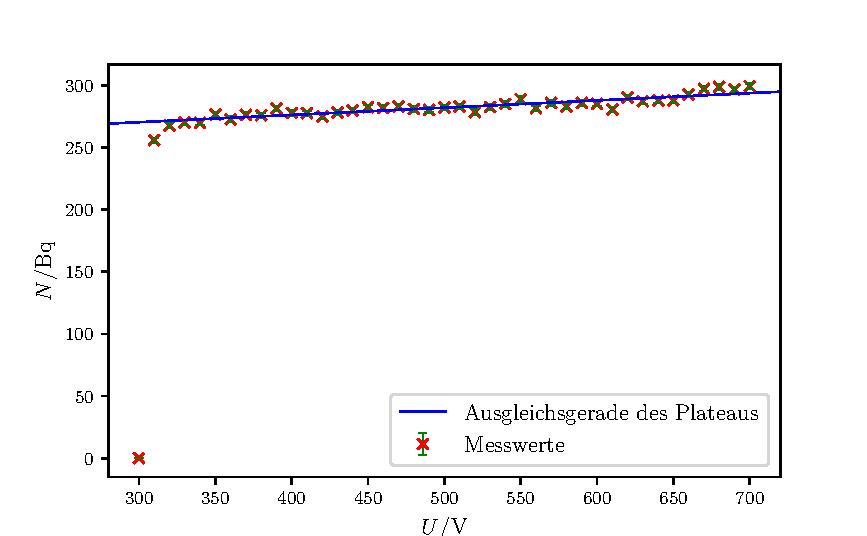
\includegraphics[width=\linewidth-50pt,height=\textheight-50pt,keepaspectratio]{content/images/Graph1.1.pdf}
	\caption{Die Impulsrate $N$ in Abhängigkeit von der Spannung $U$.}
	\label{fig:Graph1.1}
\end{figure}

\begin{figure}
	\centering
	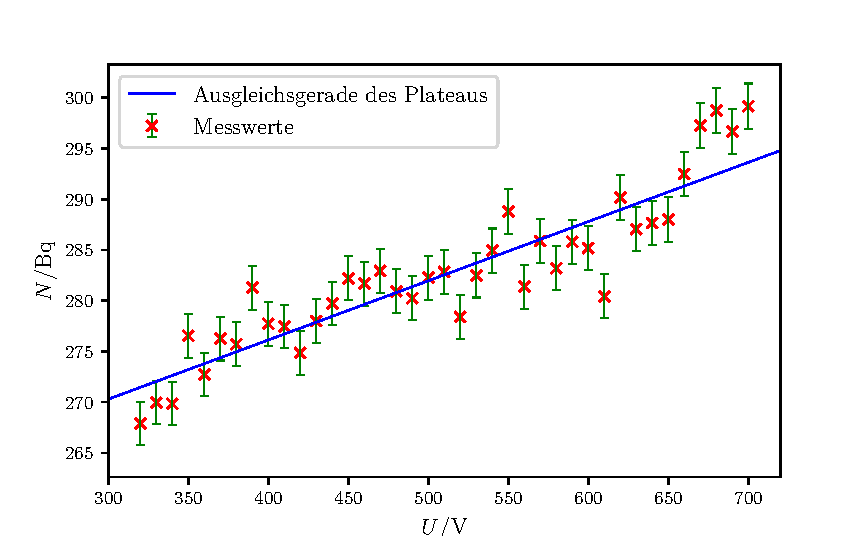
\includegraphics[width=\linewidth-50pt,height=\textheight-50pt,keepaspectratio]{content/images/Graph1.2.pdf}
	\caption{Die Impulsrate $N$ in Abhängigkeit von der Spannung $U$ im Plateaubereich.}
	\label{fig:Graph1.2}
\end{figure}

\subsection{Bestimmung der Totzeit}

Bei $U=\SI{500}{\volt}$ lässt sich am Oszilloskop eine Totzeit von $T_1=\SI{100(25)e-6}{\second}$ ablesen. Die Erholungszeit bei $U=\SI{600}{\volt}$ wird zu $T_.E=\SI{225e-6}{\second}$ abgeschätzt.\\
Bei der Zweiquellenmethode kann die Totzeit nach Formel \eqref{eq:T} berechnet werden. Dabei sind $N_1$ die Impulsrate der ersten, $N_2$ die der zweiten und $N_{1+2}$ die Impulsrate beider Quellen und haben die Werte:
\begin{align*}
N_1 	&= \SI{286(2)}{\becquerel}\\
N_2 	&= \SI{18(1)}{\becquerel}\\
N_{1+2}	&= \SI{302(2)}{\becquerel}
\end{align*} 
Somit ergibt sich für $T$:
\begin{equation*}
T_2 = \SI{120(310)e-6}{\second}
\end{equation*}
Der Fehler $\sigma_{T_2}$ von $T_2$ berechnet sich dabei nach der Gaußschen Fehlerfortpflanzung:
\begin{equation}
\sigma_{T_2} = \sqrt{\left(\frac{N_{1+2}-N_2}{2N_1^2N_2}\sigma_{N_1}\right)^2+\left(\frac{N_{1+2}-N_1}{2N_1N_2^2}\sigma_{N_2}\right)^2+\left(\frac{1}{2N_1N_2}\sigma_{N_{1+2}}\right)^2}
\end{equation}



\subsection{Bestimmung der freigesetzten Ladungsmenge pro einfallendem Teilchen}

Nach Formel \eqref{eq:I} berechnet sich die freigesetzte Ladungsmenge mit:
\begin{equation*}
\Delta Q = \frac{I}{N} \text{.}
\end{equation*}
Die Ergebnisse sind in Tabelle \ref{tab:tab1} eingetragen. In Abbildung \ref{fig:Graph2} ist $\Delta Q$ gegen $U$ aufgetragen und es wurde eine lineare Ausgleichsrechnung der Form $\Delta Q(U) = mU+Q_0$ ausgeführt um die Linearität zu überprüfen. 

\begin{figure}
	\centering
	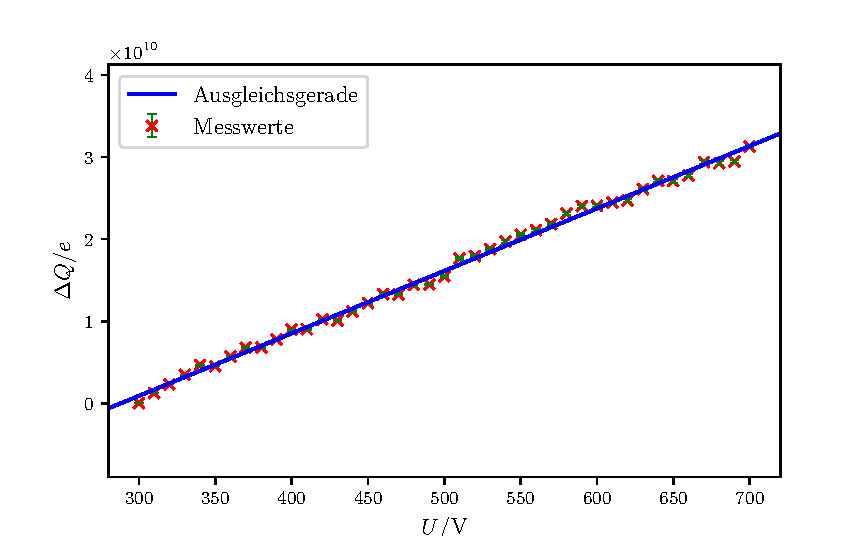
\includegraphics[width=\linewidth-50pt,height=\textheight-50pt,keepaspectratio]{content/images/Graph2.pdf}
	\caption{Die pro Teilchen freigesetzte Ladungsmenge $\Delta Q$ in Abhängigkeit von der Spannung $U$.}
	\label{fig:Graph2}
\end{figure}